\documentclass[12pt, twoside]{article}
\usepackage[letterpaper, margin=1in, headsep=0.5in]{geometry}
\usepackage[english]{babel}
\usepackage[utf8]{inputenc}
\usepackage{amsmath}
\usepackage{amsfonts}
\usepackage{amssymb}
\usepackage{tikz}
\usetikzlibrary{quotes, angles}
\usepackage{graphicx}
%\usepackage{pgfplots}
%\pgfplotsset{width=10cm,compat=1.9}
%\usepgfplotslibrary{statistics}
%\usepackage{pgfplotstable}
%\usepackage{tkz-fct}
%\usepackage{venndiagram}

\usepackage{fancyhdr}
\pagestyle{fancy}
\fancyhf{}
\renewcommand{\headrulewidth}{0pt} % disable the underline of the header

\fancyhead[RE]{\thepage}
\fancyhead[RO]{\thepage \\ Name: \hspace{3cm}}
\fancyhead[L]{BECA / Dr. Huson / Geometry 10th Grade\\* Unit 2: Midpoints and distance \\ 
18 September 2019}

\begin{document}
  \subsubsection*{2.3 Homework: Triangle area formula}
    \begin{enumerate}


   \item Find the area of $\triangle ABC$,  $Area= \frac{1}{2}bh$. The altitude $h$ of the triangle is 3 centimeters and the base $AB=6$ cm.\\[0.5cm]
   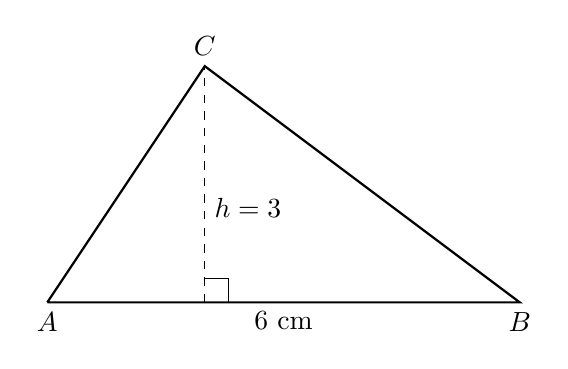
\begin{tikzpicture}[scale=1]
     \draw [thick]
       (2,0)node[below]{$A$}--
       (8,0)node[below]{$B$}--
       (4,3)node[above]{$C$} --(2,0);
    \draw [dashed] (4,0)--(4,3);
    \draw (4,0)++(0.3,0)--++(0,0.3)--+(-0.3,0);
    \node at (4,1.2)[right]{$h=3$};
    \node at (5,0)[below]{$6$ cm};
  \end{tikzpicture} \vspace{1.0cm}

  \item Find the area of $\triangle ABC$ shown below (not actual size) with $m\angle C=90^\circ$ and the lengths of the triangle's sides as $a=50$, $b=87$, and $c=100$. \\ \vspace{0.1cm}
      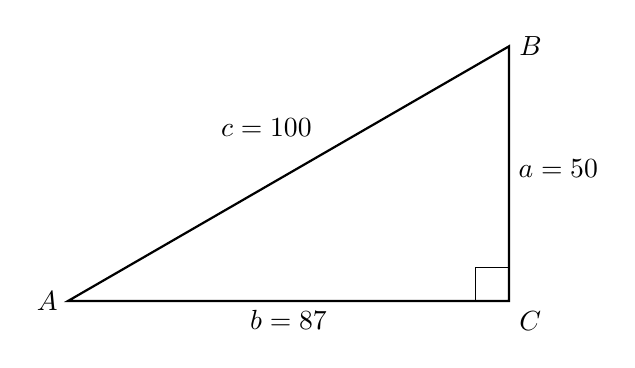
\begin{tikzpicture}[scale=1.4]
        \draw [thick]
        (0,0)node[left]{$A$}--
        (4,0)node[below right]{$C$}--
        (4,2.31)node[right]{$B$}--cycle;
        \draw (4,0)++(-0.3,0)--++(0,0.3)--+(0.3,0);
        \node at (2,0)[below]{$b=87$};
        \node at (4,1.2)[right]{$a=50$};
        \node at (1.8,1.4)[above]{$c=100$};
      \end{tikzpicture}
  \vspace{2.5cm}

  \item Draw and label a triangle $\triangle ABC$ with base $\overline{AB}$ 8 centimeters long and altitude of 5 centimeters. (show the altitude as a dotted line, and make sure it is perpendicular to the base) 

\newpage

  \item Given $\overleftrightarrow{JK}$ as shown on the number line. \\[20pt] % Midpoint
  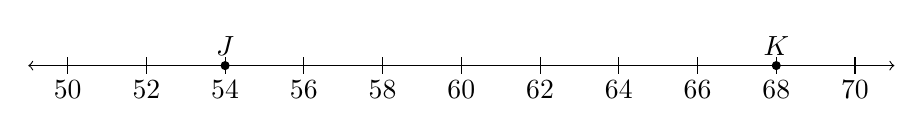
\begin{tikzpicture}[scale=0.5]
    \draw [<->] (49,0)--(71,0);
    \foreach \x in {50, 52,...,70} %2 leading for diff!=1
      \draw[shift={(\x,0)},color=black] (0pt,-6pt) -- (0pt,6pt) node[below=5pt]  {$\x$};
      \draw [fill] (54,0) circle [radius=0.1] node[above] {$J$};
      \draw [fill] (68,0) circle [radius=0.1] node[above] {$K$};
  \end{tikzpicture} \\ \bigskip
  What is the midpoint between the points $J$ and $K$? \vspace{4cm}  

  \item Given $\overline{RST}$, $S$ bisects $\overline{RT}$, $RS=17x-10$, $ST=13x-2$. Find ${RT}$.\\
  Complete all the steps for full credit.\vspace{7cm}

  \item Given $\overline{FGHI}$, $FG=8 \frac{1}{6}$, $GH=12 \frac{1}{3}$, and $HI= 5 \frac{1}{2}$. (diagram not to scale)\\ [0.25cm]
  Find ${FI}$.\\[.5in]
      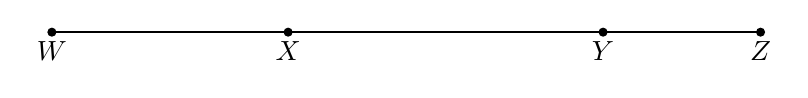
\begin{tikzpicture}
        \draw [-, thick] (0,0)--(9,0);
        \draw [fill] (0,0) circle [radius=0.05] node[below]{$W$};
        \draw [fill] (3,0) circle [radius=0.05] node[below]{$X$};
        \draw [fill] (7,0) circle [radius=0.05] node[below]{$Y$};
        \draw [fill] (9,0) circle [radius=0.05] node[below]{$Z$};
      \end{tikzpicture} \vspace{1cm}


\end{enumerate}
\end{document}


\item Given line segment $\overline{AB}$ with midpoint $M$, that is, $\overline{AM} \cong \overline{BM}$. $AB=11.8$. Find the length of $\overline{AM}$.\\[0.75cm]
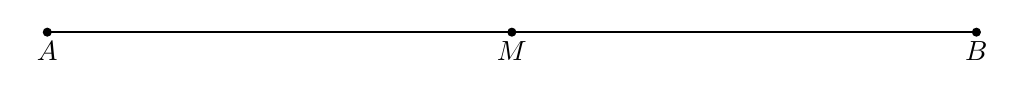
\begin{tikzpicture}
  \draw [-, thick] (0,0)--(11.8,0);
  \draw [fill] (0,0) circle [radius=0.05] node[below]{$A$};
  \draw [fill] (11.8,0) circle [radius=0.05] node[below]{$B$};
  \draw [fill] (5.9,0) circle [radius=0.05] node[below]{$M$};
\end{tikzpicture}
\vspace{3cm}
